\section{Apêndice - Gráficos com total de área ganha ano a ano por estado}

\hspace{13pt} Os gráficos a seguir mostram os anos que mais houveram ganho de área para cada estado presente no bioma. O valor da área está em metros quadrados. Os gráficos representam apenas eventos que iniciaram a partir de 1987 e não 1986, já que a maior parte dos eventos acabou ficando concentrada no primeiro ano, o que significa que a maior parte dos eventos de ganho detectados são eventos de longa duração. 

\begin{figure}[H]
    \centering
    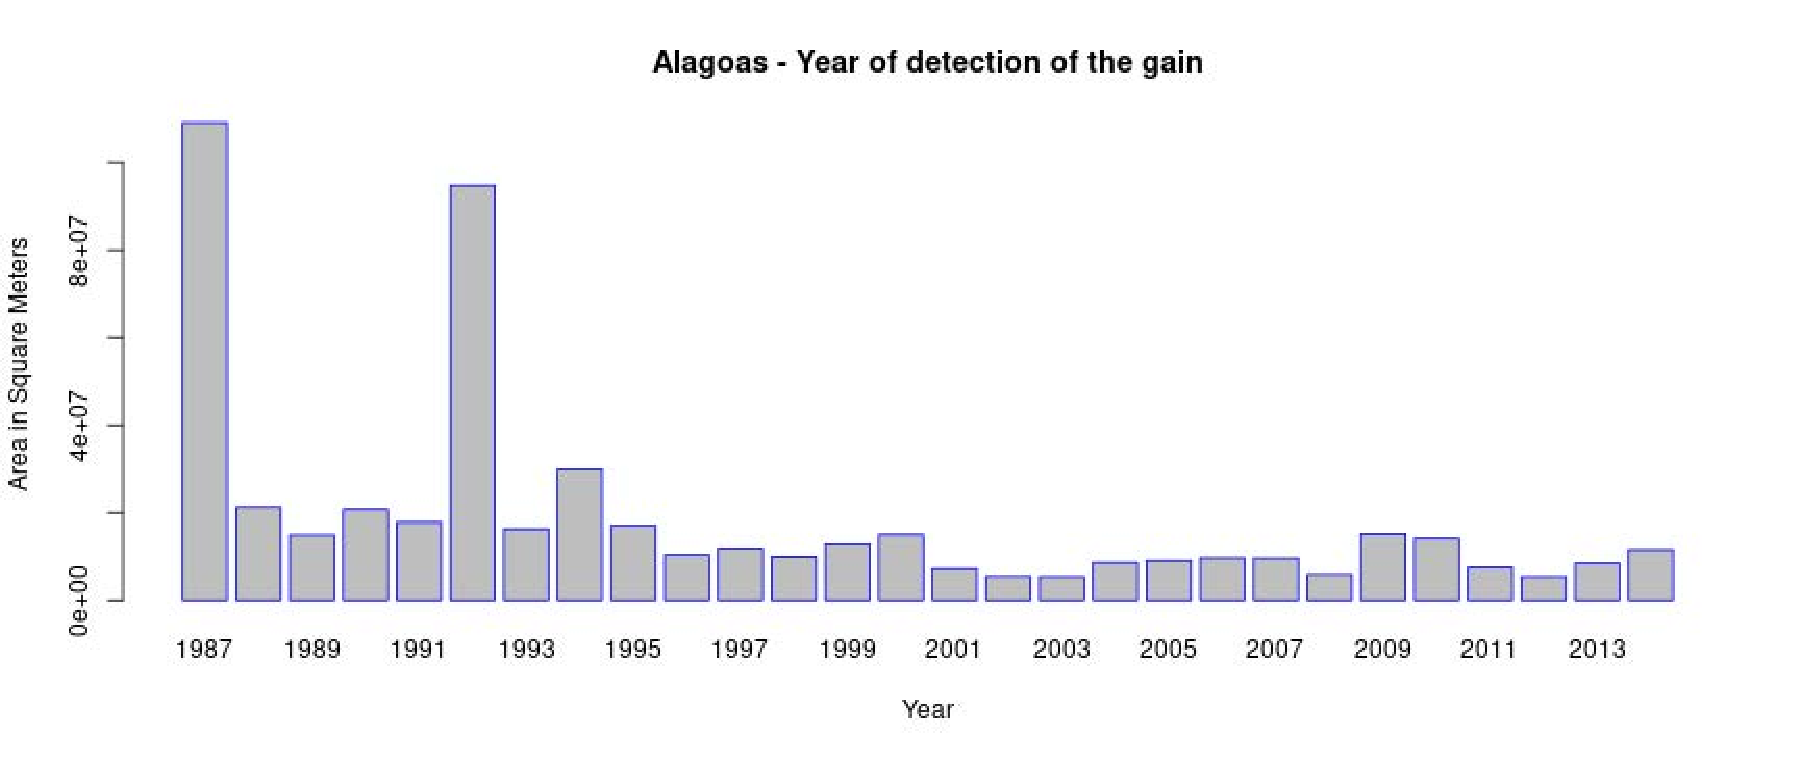
\includegraphics[scale=.5]{images/gain_graphics/Alagoas_gain.pdf}
    \caption{Ganho de área por ano em Alagoas}
    \label{fig:gain_alagoas}
\end{figure}

\begin{figure}[H]
    \centering
    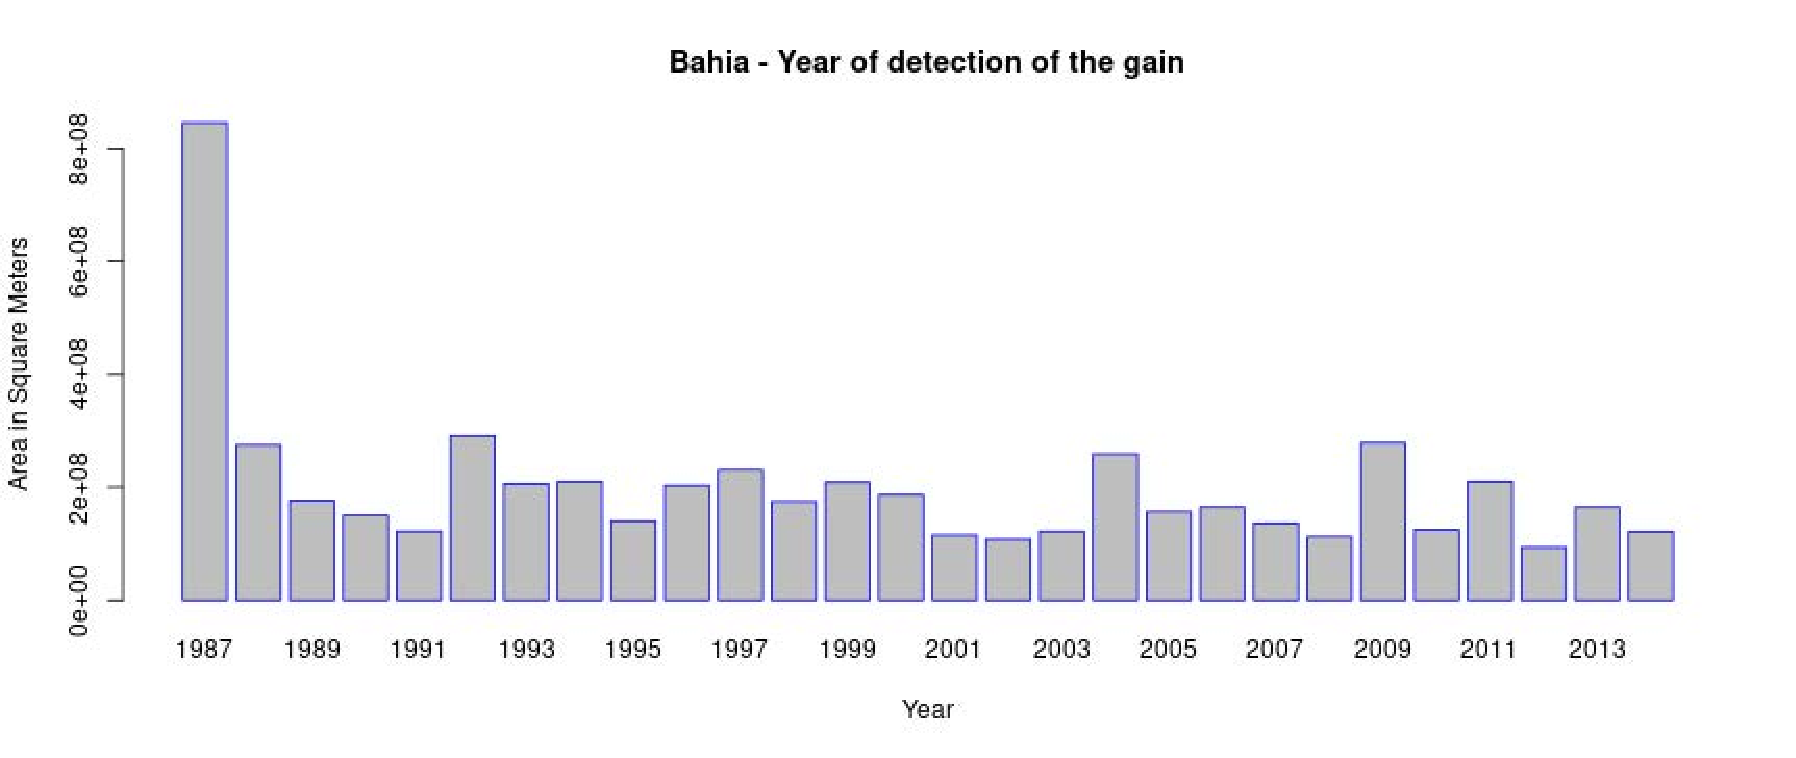
\includegraphics[scale=.5]{images/gain_graphics/Bahia_gain.pdf}
    \caption{Ganho de área por ano na Bahia}
    \label{fig:gain_bahia}
\end{figure}

\begin{figure}[H]
    \centering
    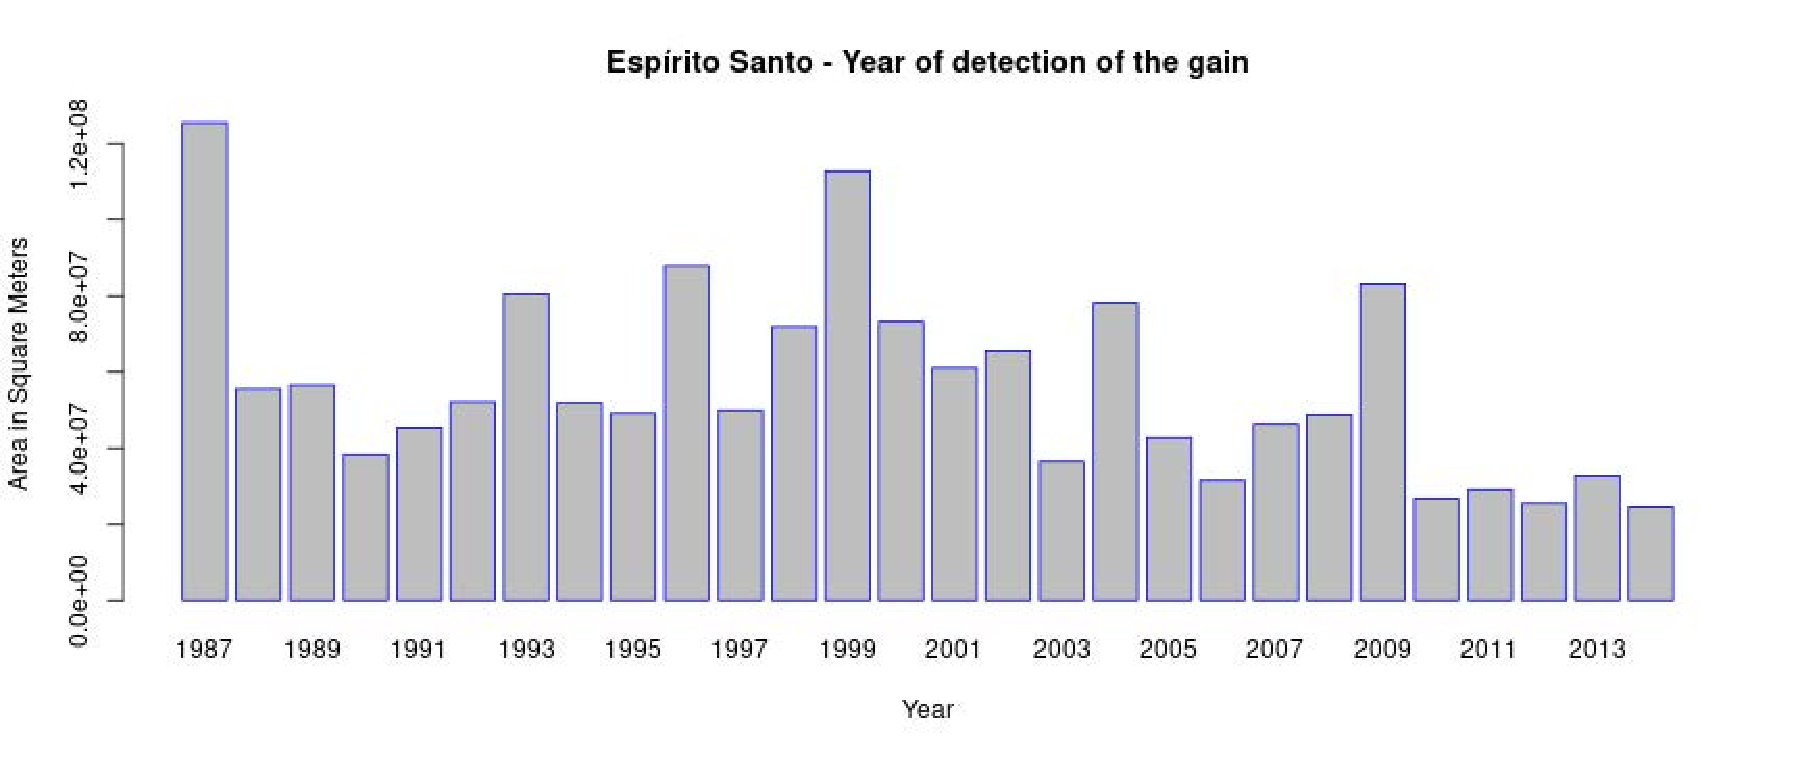
\includegraphics[scale=.5]{images/gain_graphics/Espirito_Santo_gain.pdf}
    \caption{Ganho de área por ano no Espírito Santo}
    \label{fig:gain_espirito_santo}
\end{figure}

\begin{figure}[H]
    \centering
    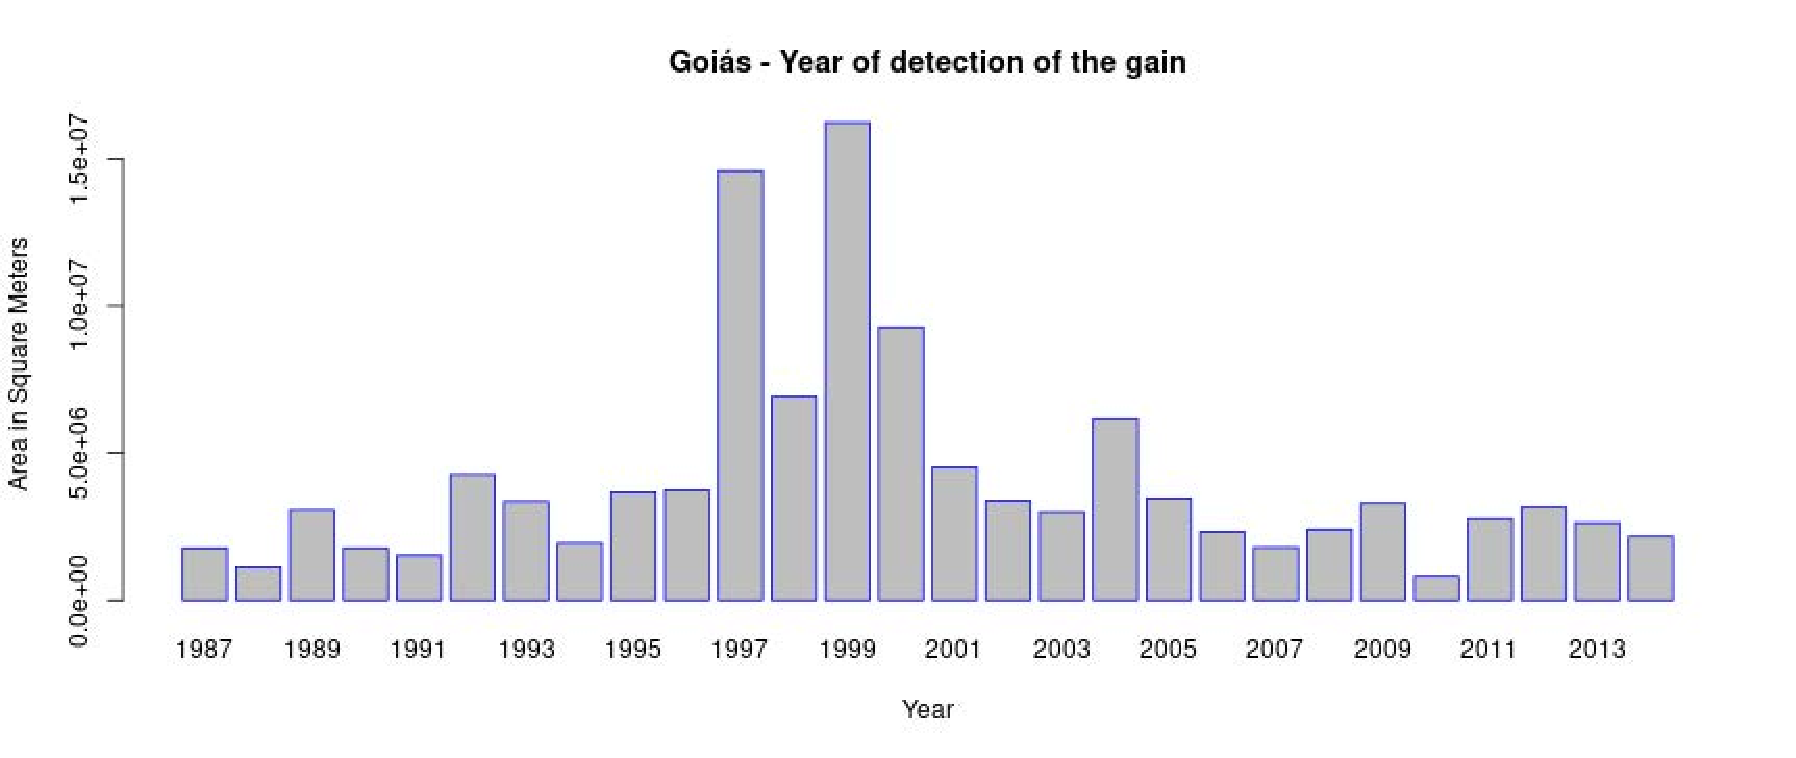
\includegraphics[scale=.5]{images/gain_graphics/Goias_gain.pdf}
    \caption{Ganho de área por ano em Goiás}
    \label{fig:gain_goias}
\end{figure}

\begin{figure}[H]
    \centering
    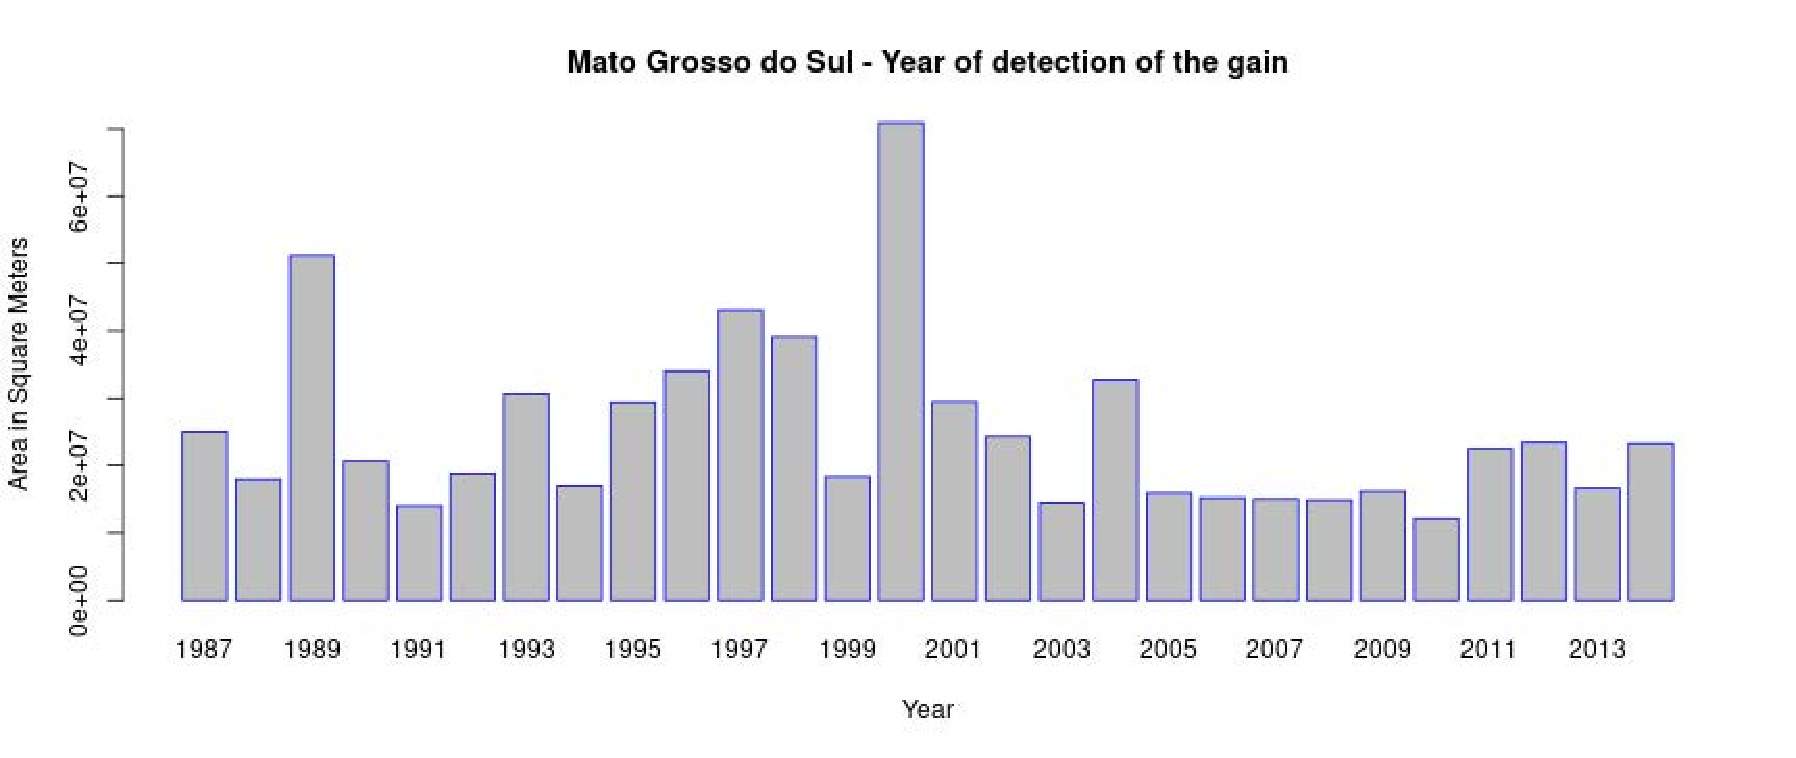
\includegraphics[scale=.5]{images/gain_graphics/Mato Grosso do Sul_gain.pdf}
    \caption{Ganho de área por ano no Mato Grosso do Sul}
    \label{fig:gain_mato_grosso_sul}
\end{figure}

\begin{figure}[H]
    \centering
    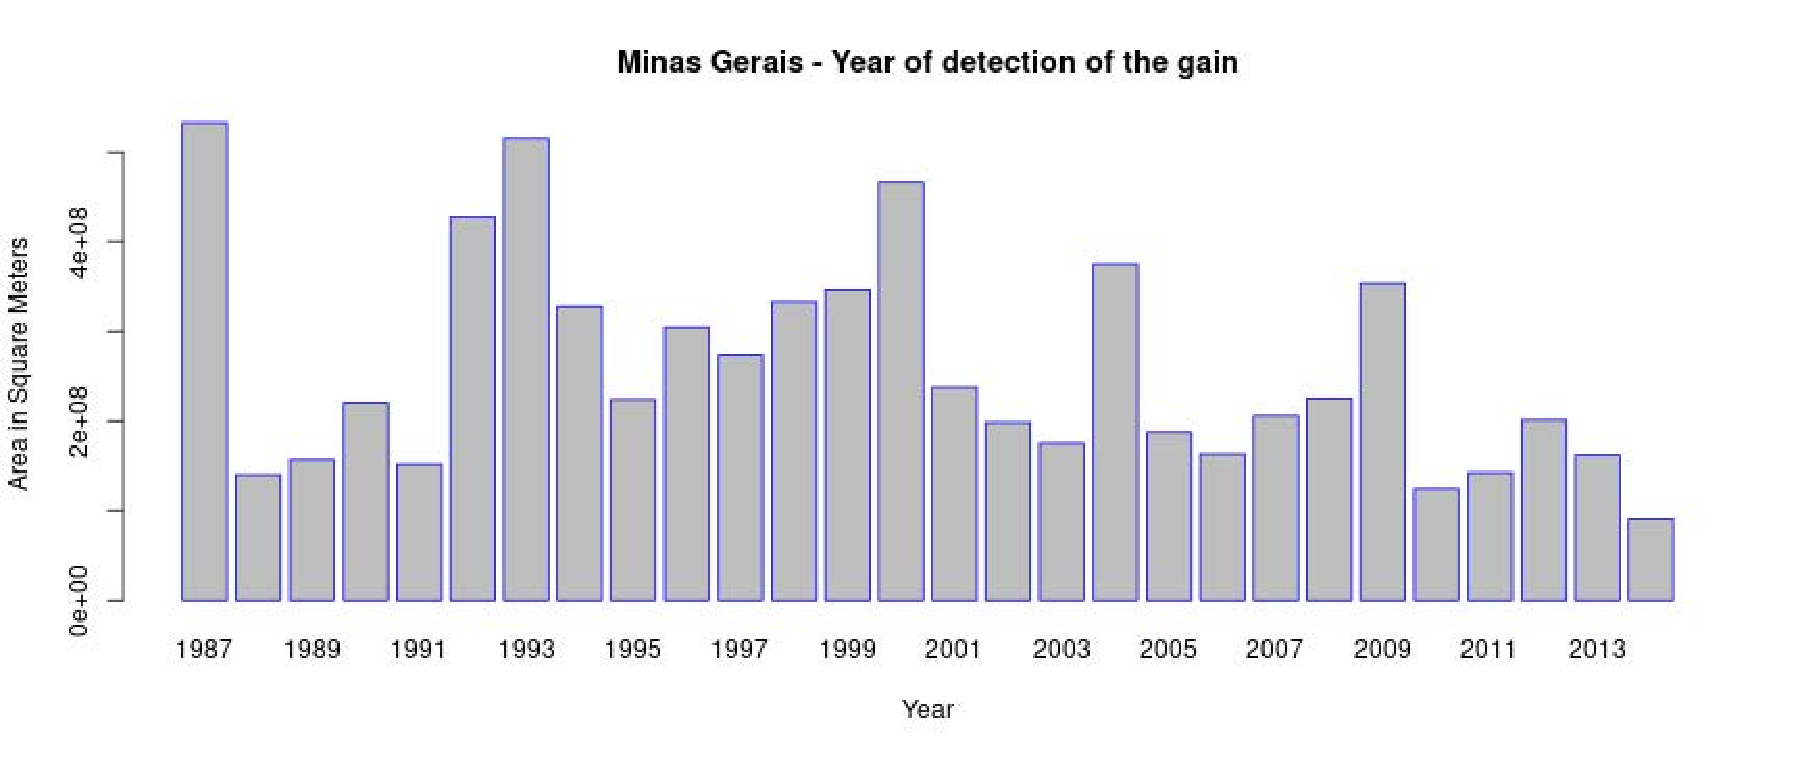
\includegraphics[scale=.5]{images/gain_graphics/Minas Gerais_gain.pdf}
    \caption{Ganho de área por ano em Minas Gerais}
    \label{fig:gain_minas_gerais}
\end{figure}

\begin{figure}[H]
    \centering
    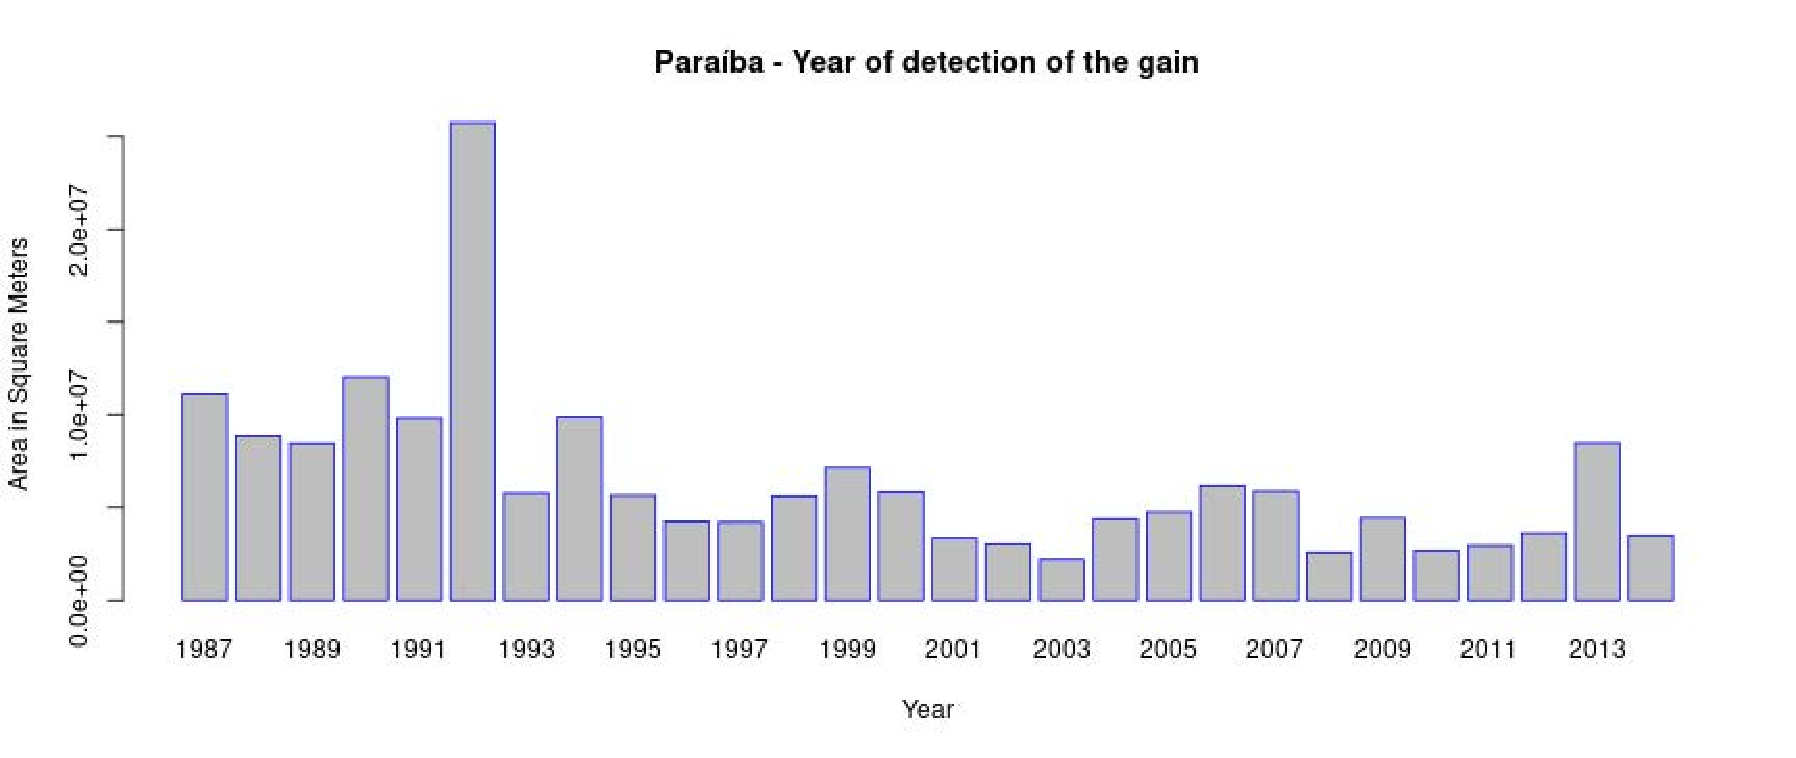
\includegraphics[scale=.5]{images/gain_graphics/Paraiba_gain.pdf}
    \caption{Ganho de área por ano na Paraíba}
    \label{fig:gain_paraiba}
\end{figure}

\begin{figure}[H]
    \centering
    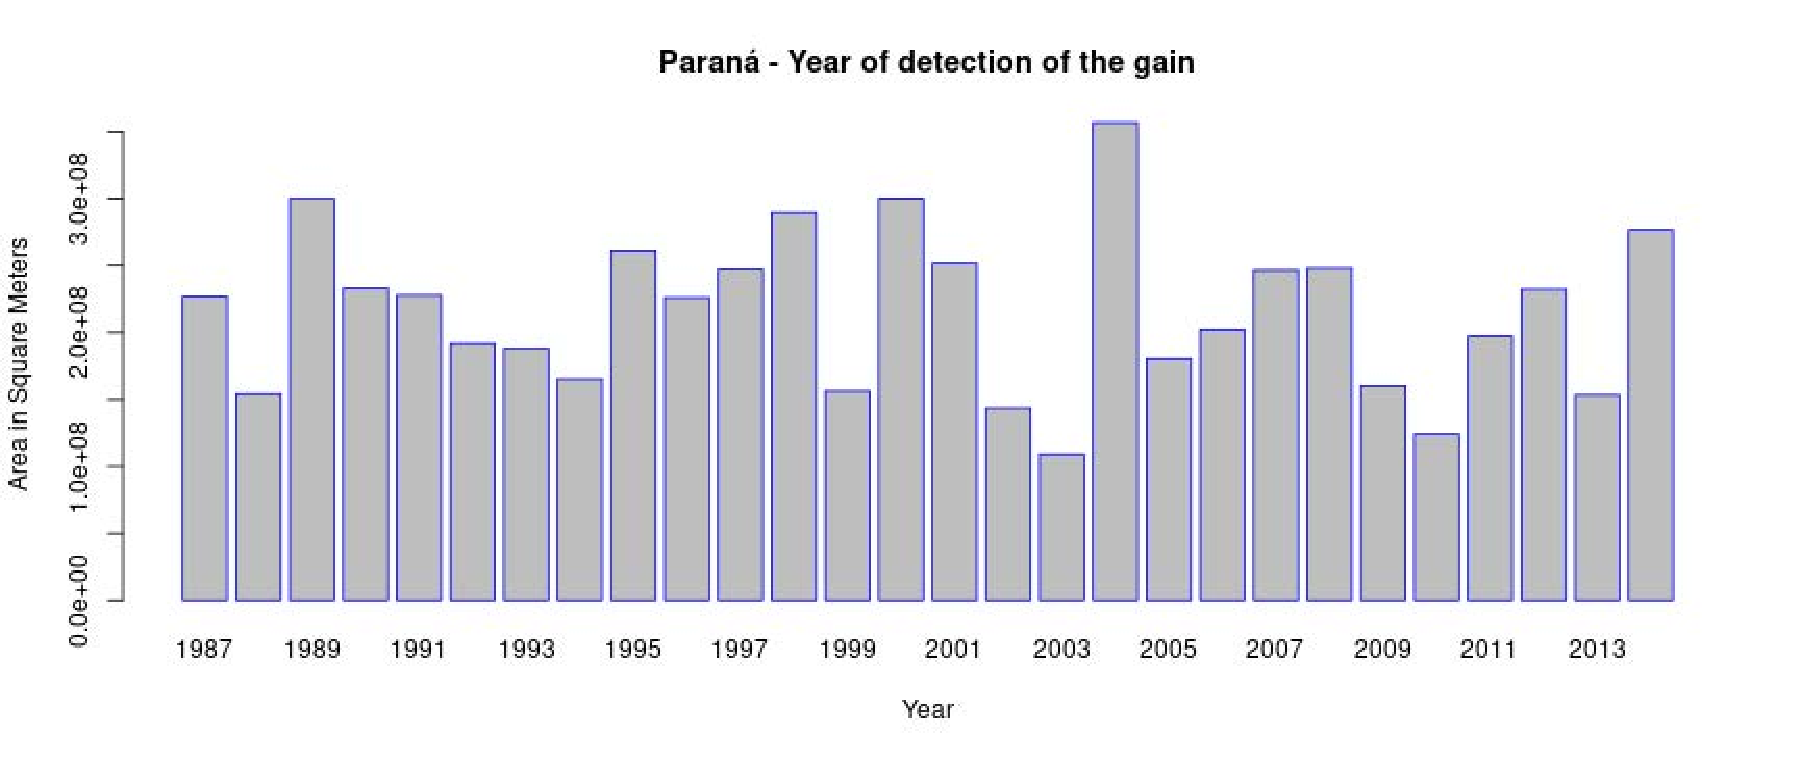
\includegraphics[scale=.5]{images/gain_graphics/Parana_gain.pdf}
    \caption{Ganho de área por ano no Paraná}
    \label{fig:gain_parana}
\end{figure}

\begin{figure}[H]
    \centering
    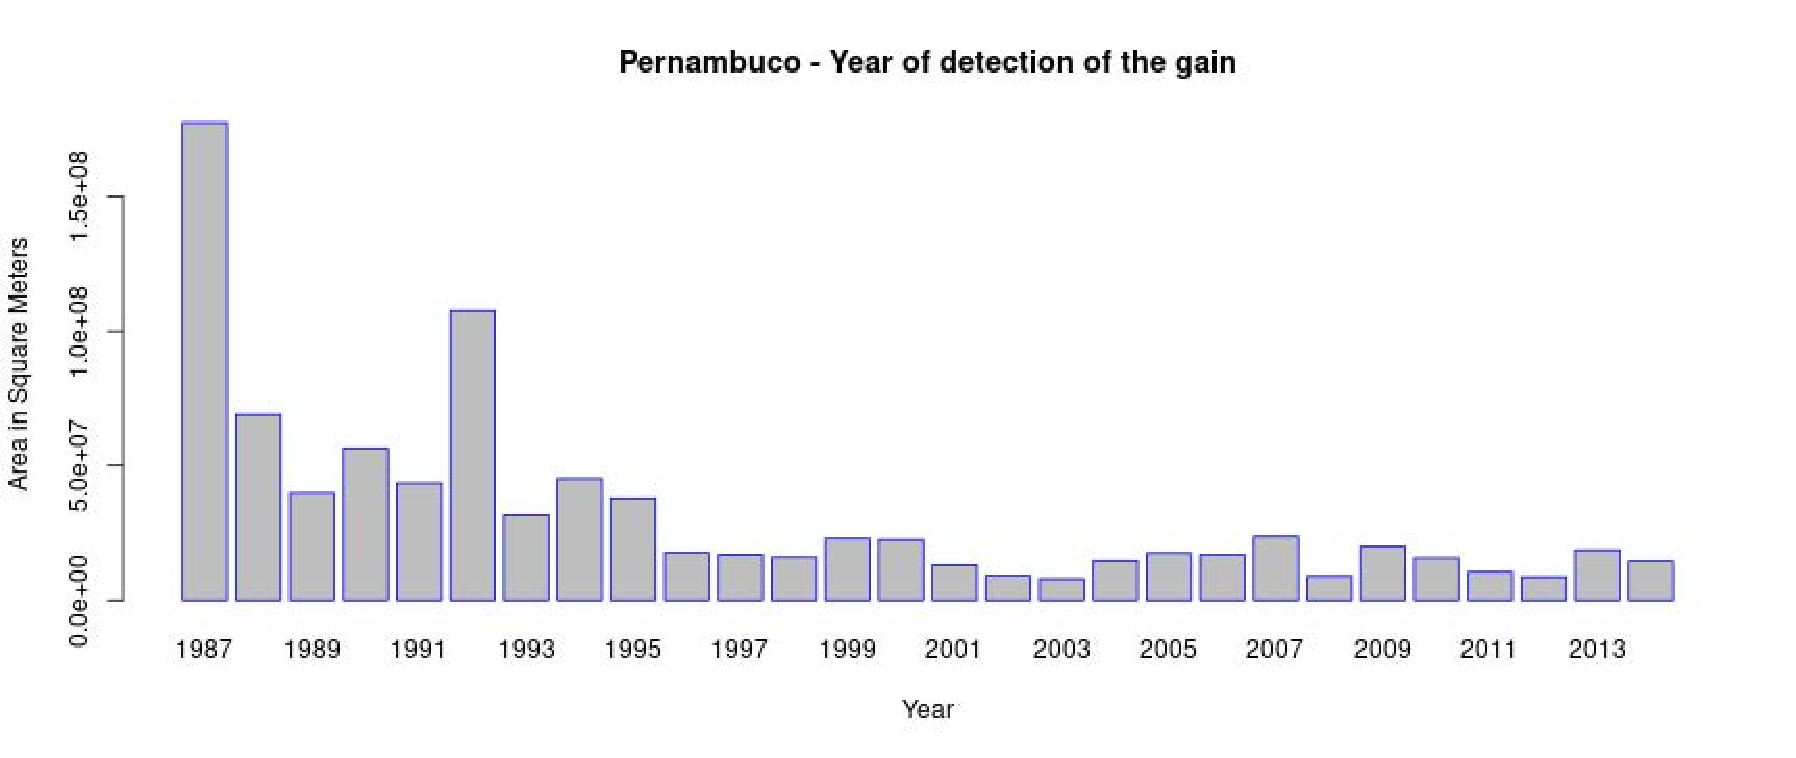
\includegraphics[scale=.5]{images/gain_graphics/Pernambuco_gain.pdf}
    \caption{Ganho de área por ano em Pernambuco}
    \label{fig:gain_pernambuco}
\end{figure}

\begin{figure}[H]
    \centering
    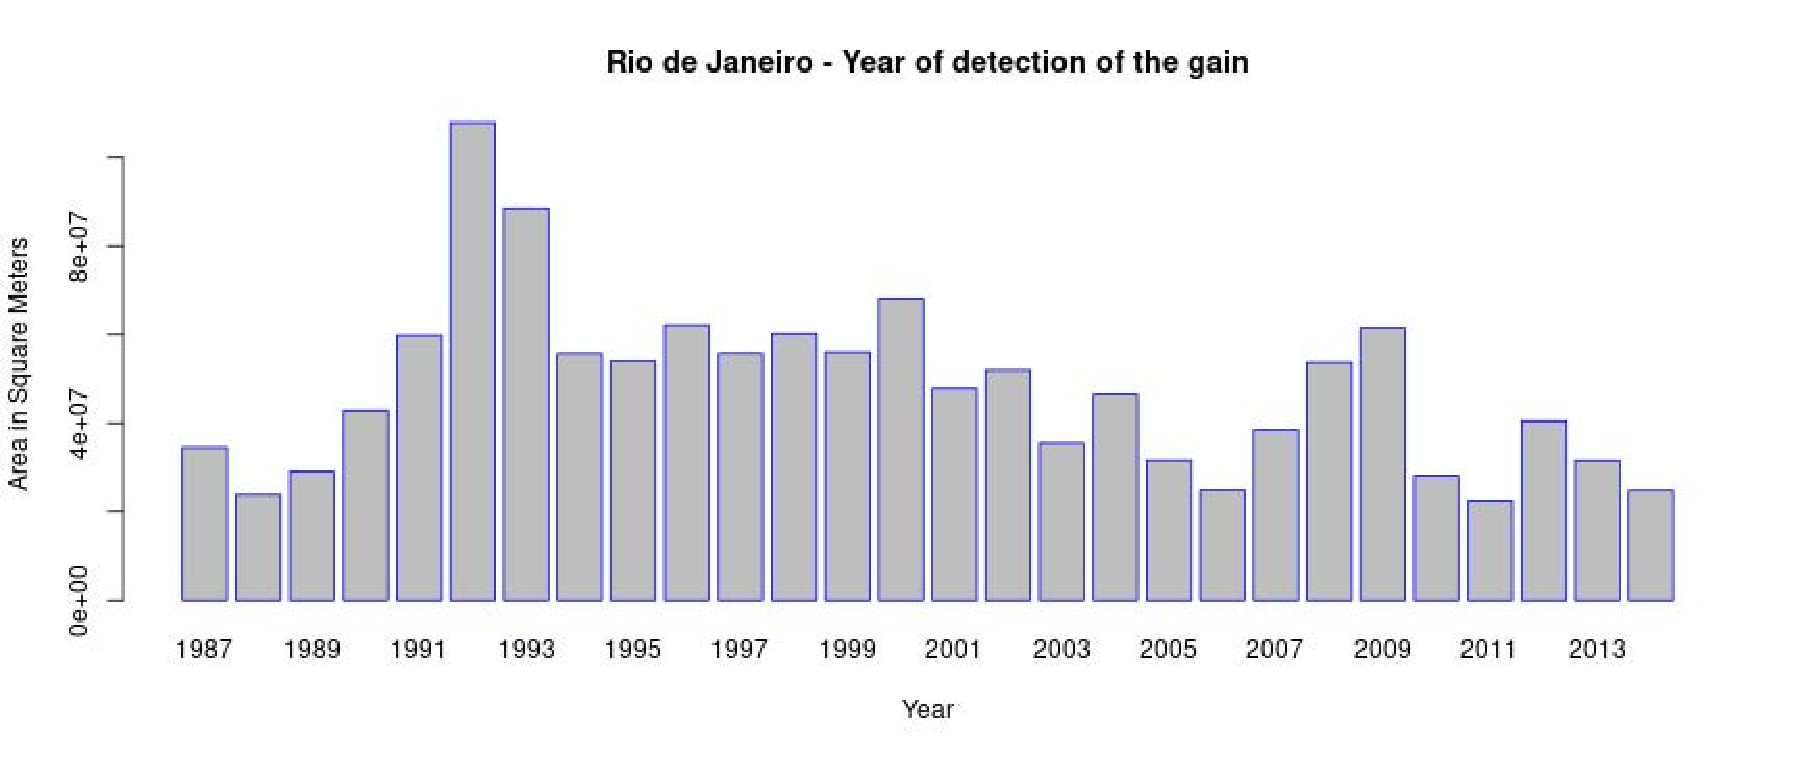
\includegraphics[scale=.5]{images/gain_graphics/Rio de Janeiro_gain.pdf}
    \caption{Ganho de área por ano no Rio de Janeiro}
    \label{fig:gain_rio_de_janeiro}
\end{figure}

\begin{figure}[H]
    \centering
    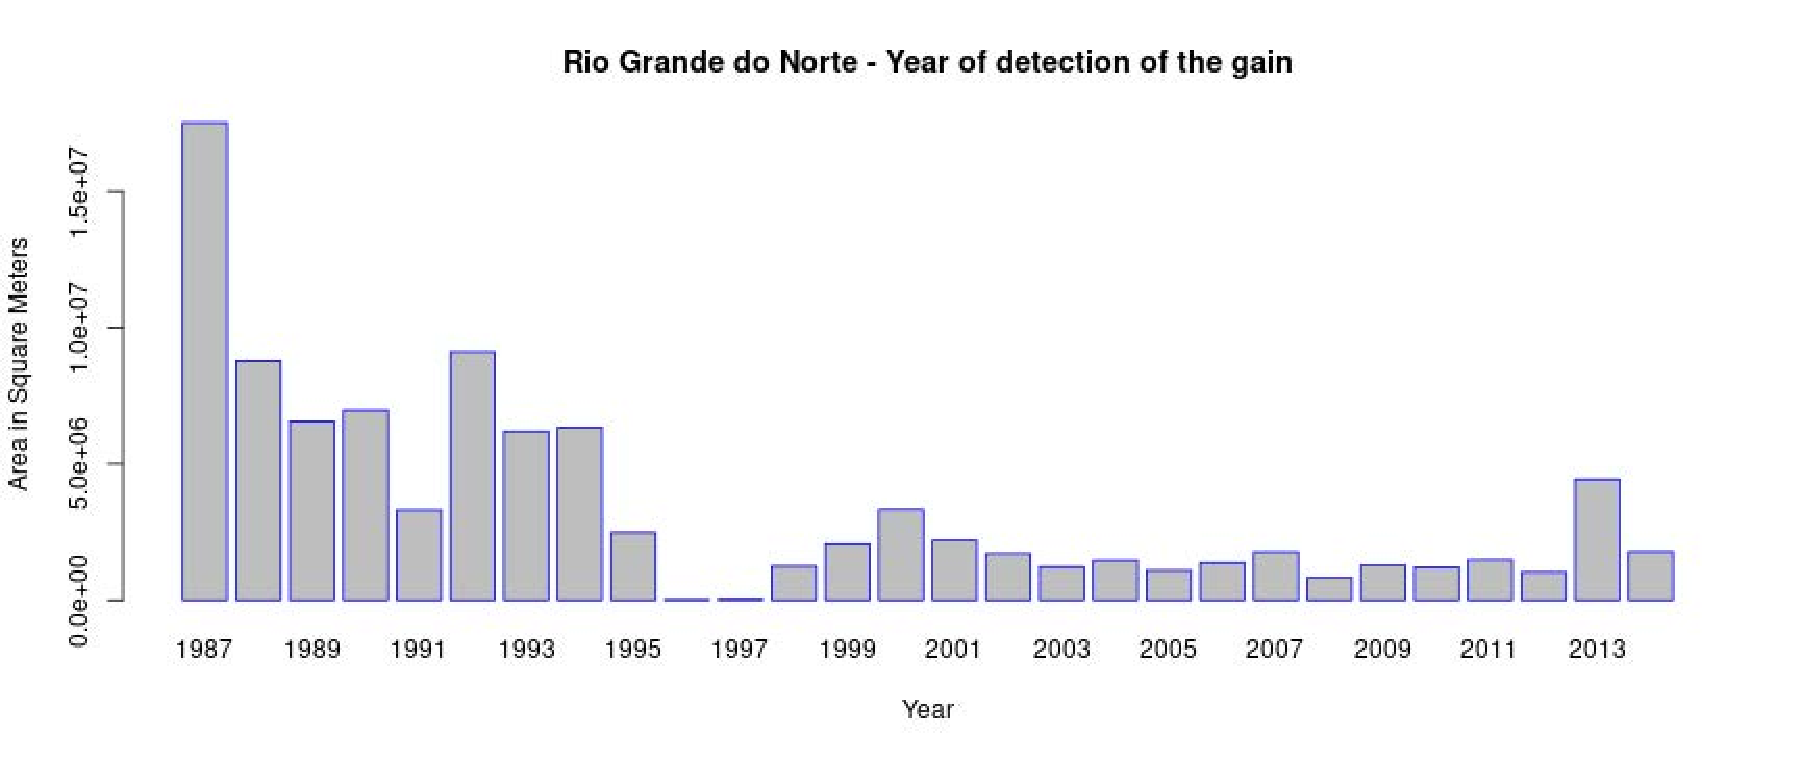
\includegraphics[scale=.5]{images/gain_graphics/Rio Grande do Norte_gain.pdf}
    \caption{Ganho de área por ano no Rio Grande do Norte}
    \label{fig:gain_rio_grande_do_norte}
\end{figure}

\begin{figure}[H]
    \centering
    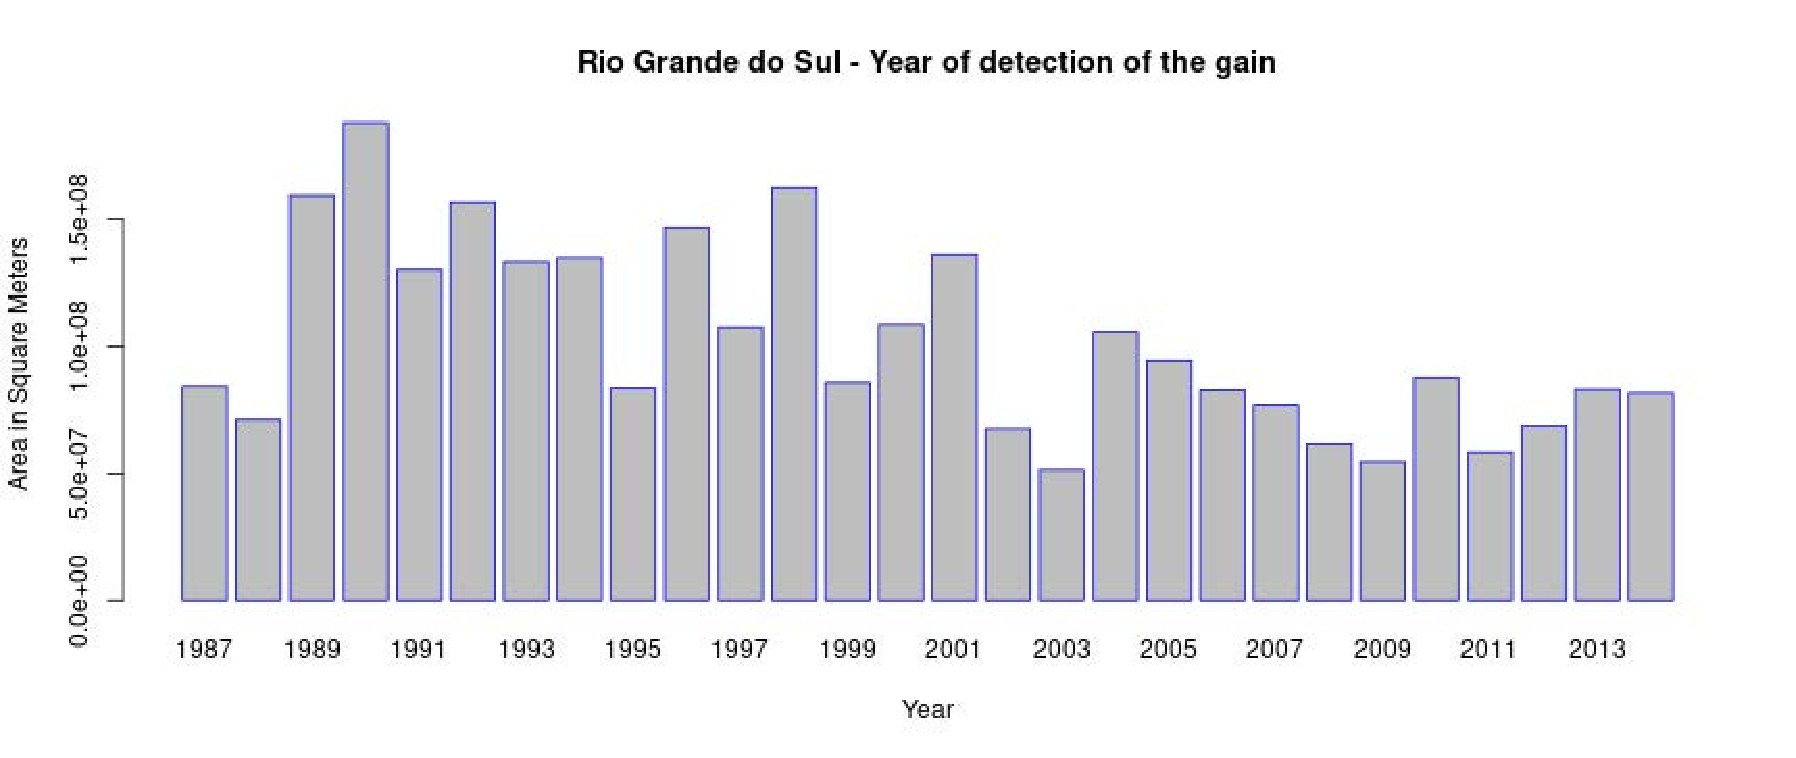
\includegraphics[scale=.5]{images/gain_graphics/Rio Grande do Sul_gain.pdf}
    \caption{Ganho de área por ano no Rio Grande do Sul}
    \label{fig:gain_rio_grande_do_sul}
\end{figure}

\begin{figure}[H]
    \centering
    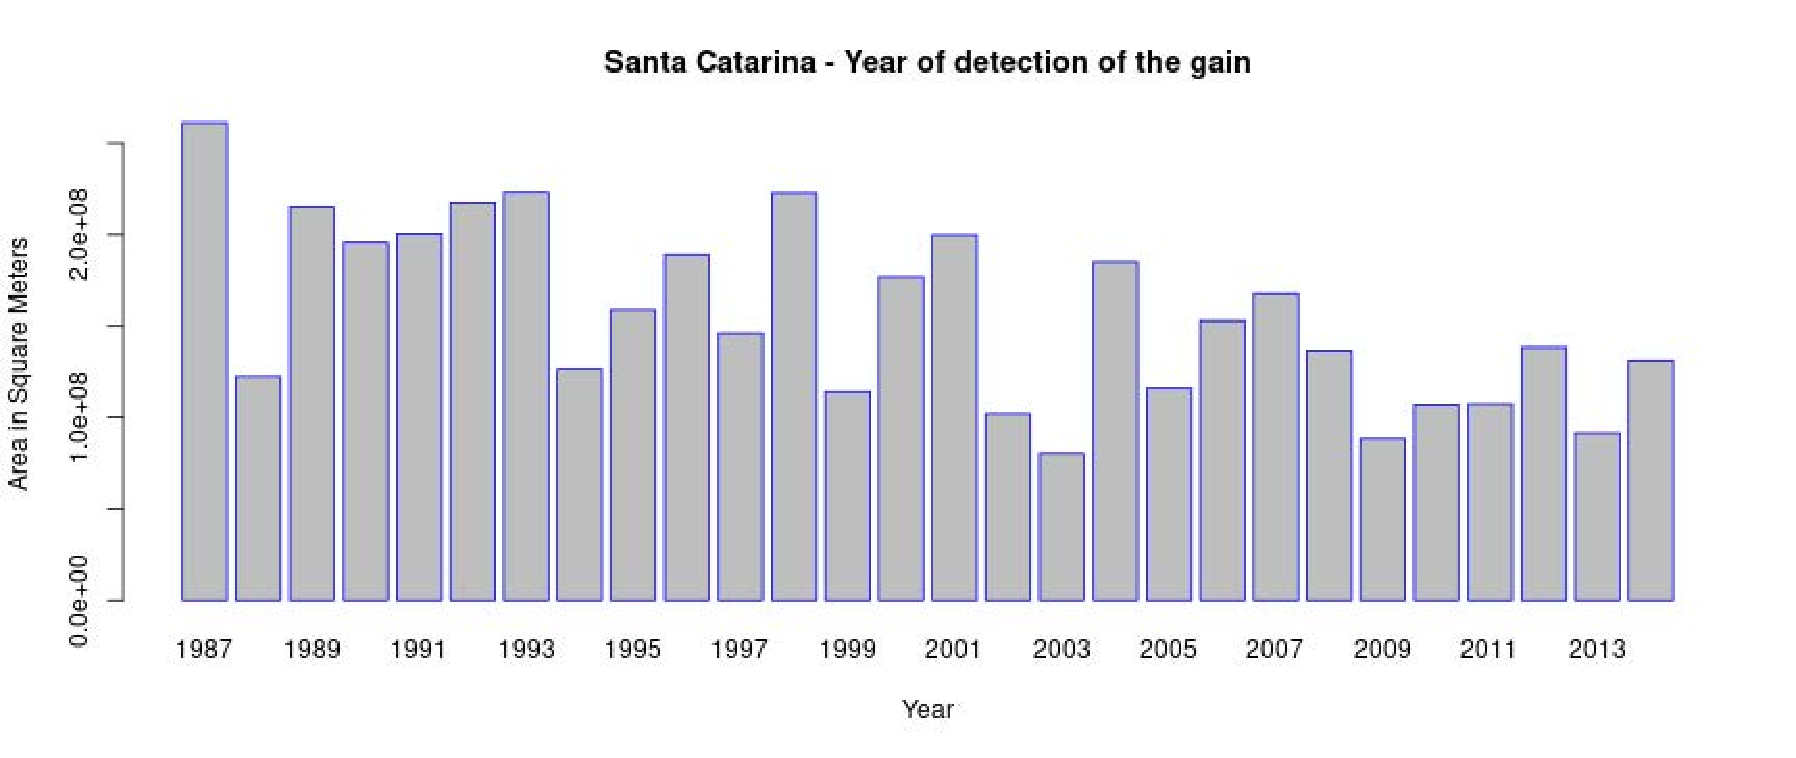
\includegraphics[scale=.5]{images/gain_graphics/Santa Catarina_gain.pdf}
    \caption{Ganho de área por ano em Santa Catarina}
    \label{fig:gain_santa_catarina}
\end{figure}

\begin{figure}[H]
    \centering
    \includegraphics[scale=.5]{images/gain_graphics/São Paulo_gain.pdf}
    \caption{Ganho de área por ano em São Paulo}
    \label{fig:gain_sao_paulo}
\end{figure}

\begin{figure}[H]
    \centering
    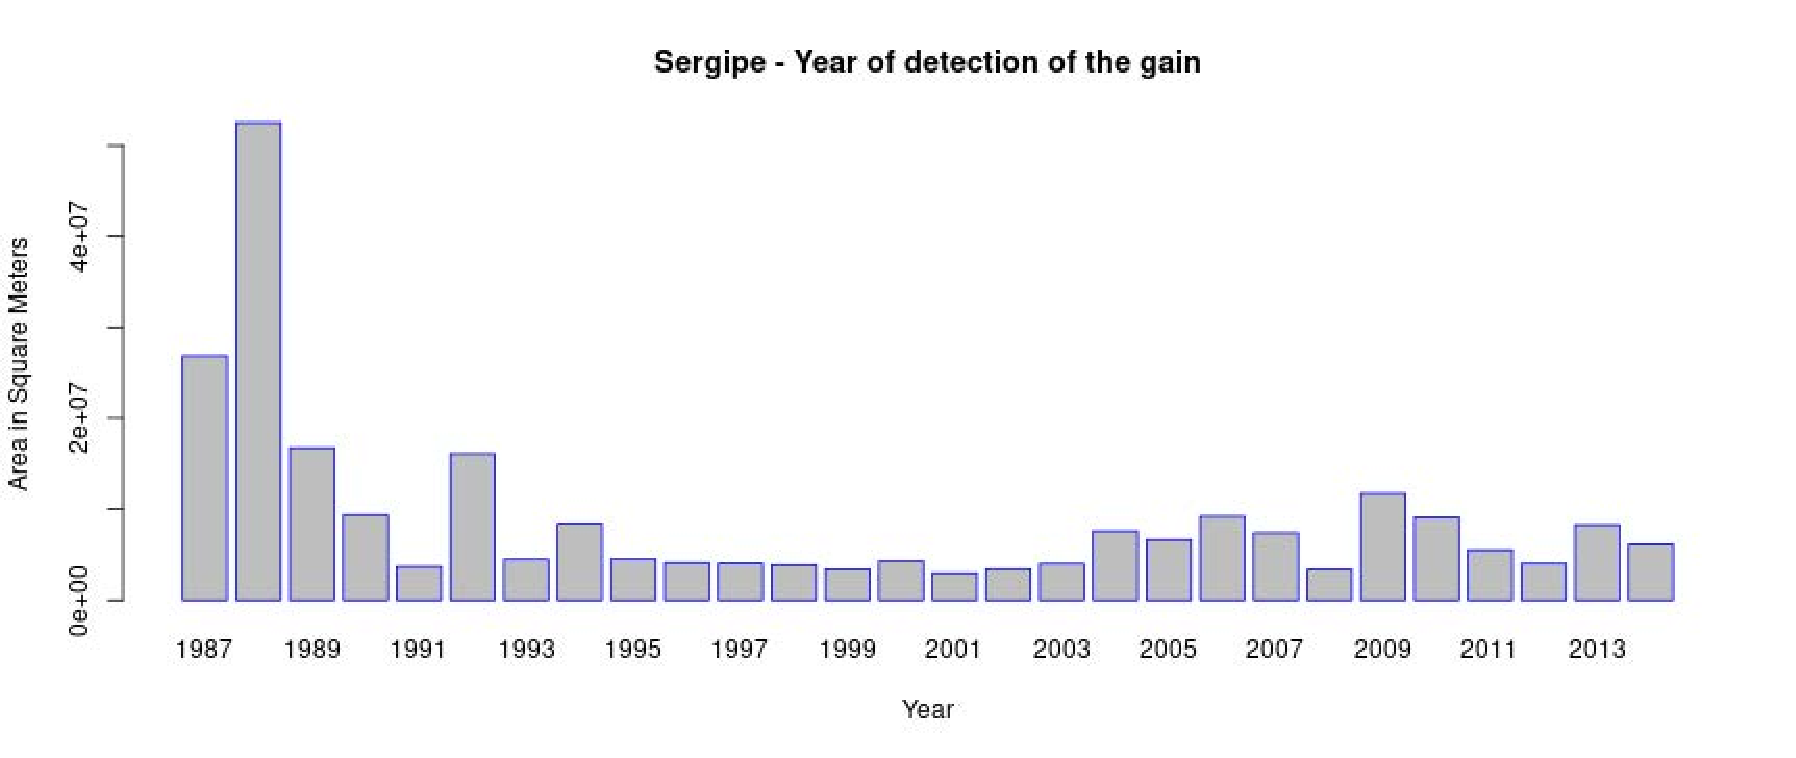
\includegraphics[scale=.5]{images/gain_graphics/Sergipe_gain.pdf}
    \caption{Ganho de área por ano em Sergipe}
    \label{fig:gain_sergipe}
\end{figure}